\documentclass[12pt,onecolumn,a4paper]{article}
\usepackage{epsfig,graphicx,subfigure,amsthm,amsmath}
\usepackage{color,xcolor}   
\usepackage{hyperref}
\usepackage{xepersian}
\settextfont[Scale=1.2]{BZAR.TTF}
\setlatintextfont[Scale=1]{Times New Roman}
\renewcommand{\baselinestretch}{1.2}
\usepackage{amsmath}
\usepackage{graphicx}
\usepackage{amsthm}
\newtheorem{thm}{Theorem}
\newtheorem*{numlessthm}{Theorem}
\usepackage{color}
\usepackage{hyperref}






\begin{document}
\title{قضیه فیثاغورس} 
\author{محمدامین روشنی}
\date{\today}
\maketitle
\tableofcontents
\newpage
\section{مقدمه} 
قضیه فیثاغورس در هندسه اقلیدسی است که بر اساس آن، در یک مثلث راست‌گوشه (قائم‌الزاویه)، همواره مجموع مربع ‌های دو ضلع برابر با مربع وتر است.
\\
این قضیه به نام ریاضی‌دان یونانی فیثاغورس نامگذاری شده‌است.


\section{اثبات بااستفاده از بازچینی}
\label{sec1}
در نگاره پویای سمت چپ، مساحت کل و مساحت مثلث‌ها همگی ثابت است؛ بنابراین، مساحت کل ناحیه سیاه رنگ، ثابت است. اما ناحیه اصلی سیاه رنگ با ضلع \lr{c} را می‌توان به دو مربع با ضلع‌های \lr{a} و \lr{b} تقسیم کرد و نشان داد که: \lr{a۲} + \lr{b۲} = \lr{c۲}.

اثبات دوم با استفاده از نگاره پویای میانی است. مربع بزرگ اول، مساحتی برابر با \lr{c۲} دارد با کنار هم قرار دادن چهار مثلث راست‌گوشه یکسان و به دلیل اختلاف طول ضلع مثلث‌ها، یک مربع کوچک میان آن‌ها و در مرکز مربع بزرگ باقی می‌ماند. اگر یک بار دیگر نگاه کنیم می‌بینیم که با جابجایی مثلث‌ها، دو مستطیل با ضلع‌های \lr{a} و \lr{b} تشکیل شده‌است. با ادغام مربع کوچک میانی با یکی از مستطیل‌ها، دو مستطیل به دو مربع تبدیل خواهد شد و مساحت هریک از آن‌ها برابر با \lr{a۲} و \lr{b۲} خواهد بود؛ بنابراین \lr{c۲} = \lr{a۲} + \lr{b۲}. است.

نگاره سوم سمت راست، نیز خود یک اثبات است. همان گونه که در نگاره نمایش داده شده‌است، دو مربع بالایی، با سایه‌های آبی و سبز به چندین بخش تقسیم شده‌اند. اگر این قسمت‌های سایه‌خورده را کنار هم بچینیم می‌بینیم که مربع پایینی روی وتر را به خوبی پر می‌کنند؛ عکس این مطلب نیز برقرار است یعنی مربع پایینی که روی وتر تشکیل شده را می‌توان چنان قسمت کرد که دو مربع بالایی به خوبی با این قسمت‌ها پر شود. با این کار نشان دادیم که مساحت مربع بزرگ برابر است با مجموع مساحت‌های دو مربع کوچک..

\begin{figure}[h]
    \begin{center}
    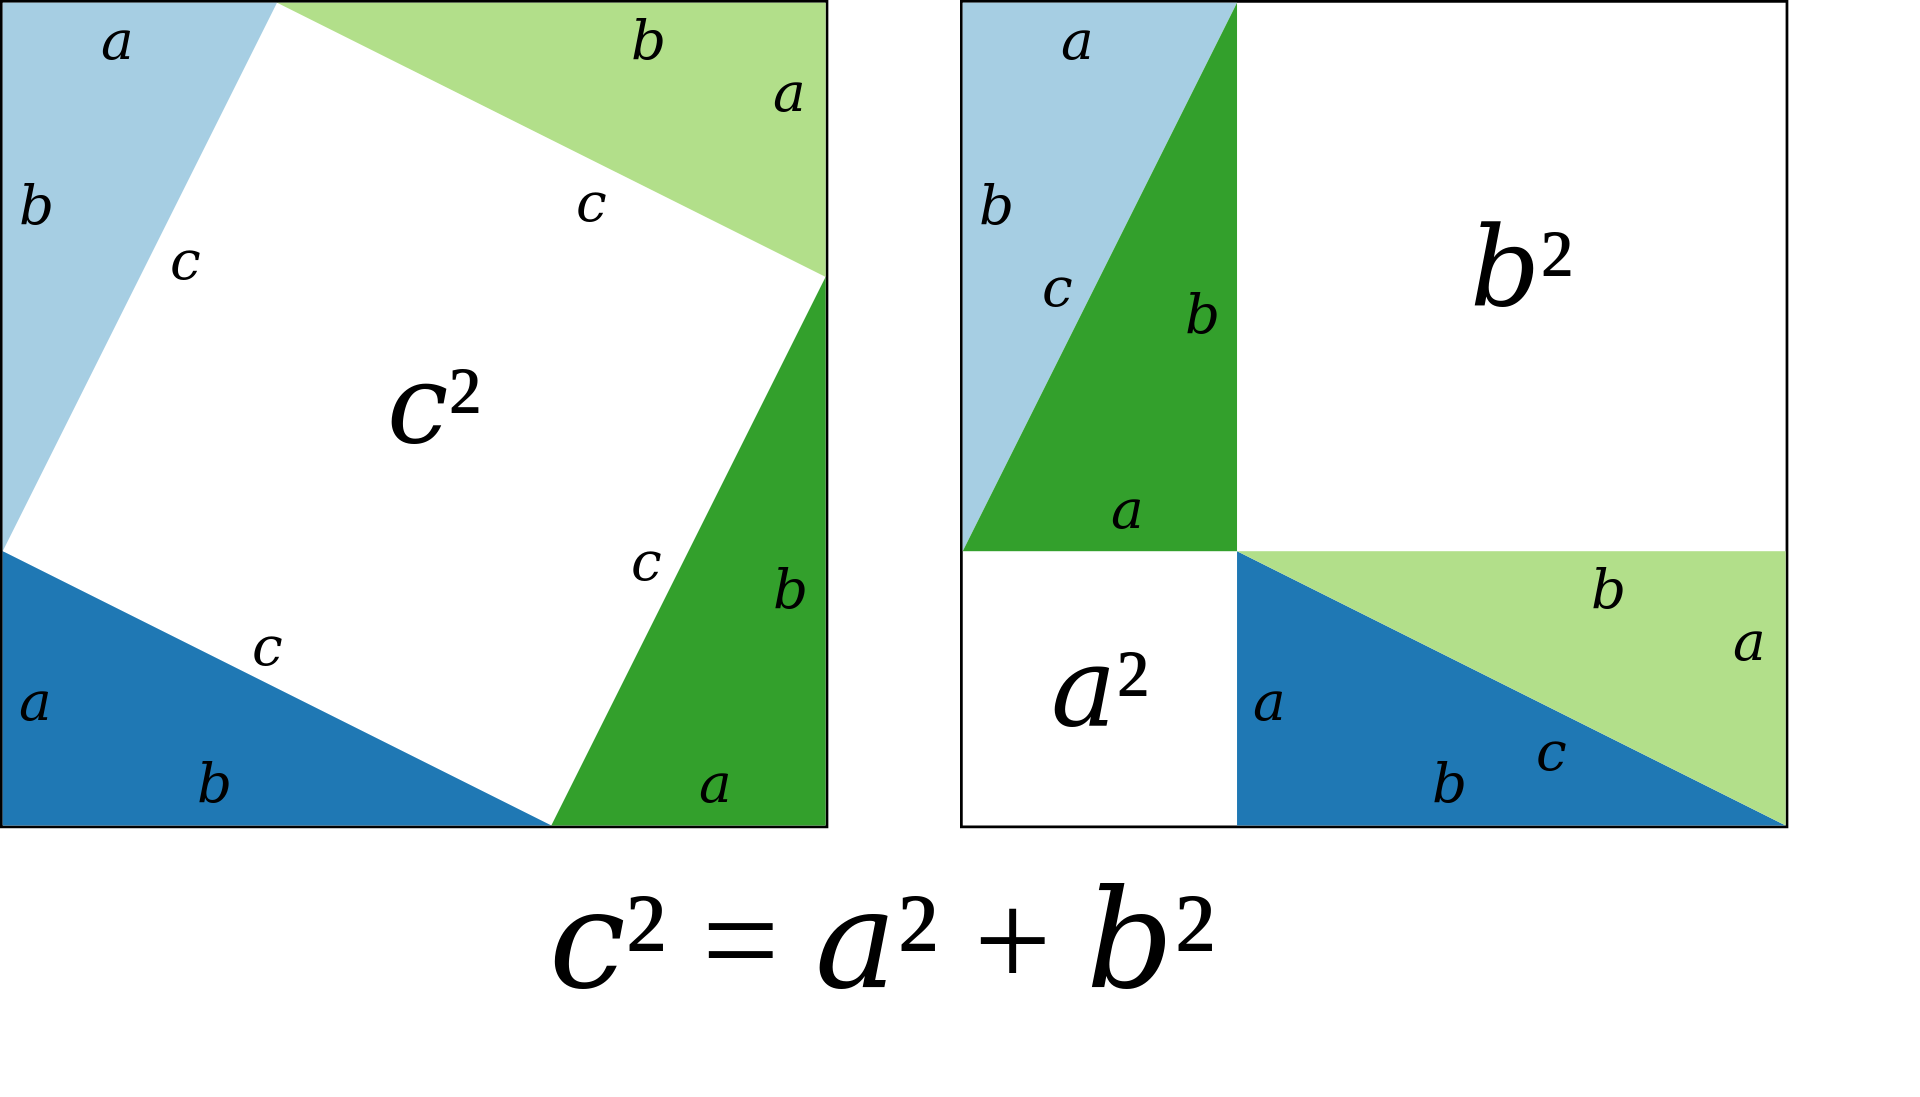
\includegraphics[scale=0.12]{figs/Pythagoras-proof-anim.svg.png} \\
    \caption{قضیه بازچینی}
    \label{fig:my_label}
    \end{center}
\end{figure}
\begin{equation}
    c = \sqrt{a^2 + b^2}
\end{equation}
\begin{equation}
    \sqrt{(a_1 + a_1)^2 + (a_2 + a_2)^2 + (a_n + a_n)^2} = \sqrt{\sum_{i=1}^{n} (a_i - b_i)^2}
\end{equation}

\subsection{توضیحات اضافی}

معادله فیثاغوریا دو طرف مثلث سمت راست را به روشی ساده مرتبط می کند ، به طوری که در صورت مشخص شدن طول هر دو طرف می توان طول طرف سوم را پیدا کرد. نتیجه دیگر قضیه این است که در هر مثلث سمت راست ، هیپوتنوز از هر یک از طرفهای دیگر بیشتر است ، اما کمتر از مبلغ آنها است.


\section{اثبات دیگر قضیه}
آلبرت انیشتین اثبات قطعه قطعه ای را نشان داد که در آن قطعات نیازی به جابجایی ندارند. به جای استفاده از یک مربع روی هیپوتنوز و دو مربع روی پاها ، می توان از هر شکل دیگری که شامل هیپوتنوز است استفاده کرد و دو شکل مشابه که هر یک به جای هیپوتنوز یکی از دو پا را شامل می شوند (به شکل های مشابه در سه طرف مراجعه کنید). . در اثبات انیشتین ، شکلی که شامل هیپوتنوز است ، خود مثلث مناسب است. برش متشکل از رها کردن عمود از راس زاویه سمت راست مثلث به هیپوتنوز است ، بنابراین کل مثلث را به دو قسمت تقسیم می کنیم. آن دو قسمت مانند مثلث راست اصلی شکل دارند و پاهای مثلث اصلی را به عنوان هیپوتنوس دارند و جمع مناطق آنها مثلث مثلث اصلی است. از آنجا که نسبت مساحت یک مثلث سمت راست به مربع هایپوتوس آن برای مثلثهای مشابه یکسان است ، رابطه بین نواحی سه مثلث برای مربع های طرفین مثلث بزرگ نیز حفظ می شود.

\section{لیست برخی از اثبات}
\begin{enumerate}
     \item اثبات استفاده از مثلثهای مشابه
    \item اثبات اقلیدس
    \item اثبات براساس قطع و تنظیم مجدد
    \item اثبات انیشتین با قطع عضو بدون تنظیم مجدد
    \item اثبات جبری
\end{enumerate}

\subsection{جدول اثبات}
\begin{center}
 \begin{tabular}{||c | c||} 
\hline
 1 & اثبات استفاده از مثلثهای مشابه \\ 
 \hline
 2 & اثبات اقلیدس \\
 \hline
 3 & اثبات براساس قطع و تنظیم مجدد \\
 \hline
 4 & اثبات انیشتین با قطع عضو بدون تنظیم مجدد \\
 \hline
 5 & اثبات جبری \\ [1ex] 
 \hline
\end{tabular}
\newline
\end{center}


    \begin{thebibliography}{1}

        \bibitem{1} {
		\lr{
            Judith D. Sally; Paul Sally (2007). "Chapter 3: Pythagorean triples". Roots to research: a vertical development of mathematical problems. American Mathematical Society Bookstore. p. 63. ISBN 0-8218-4403-2.}}
        \bibitem{2} {
		\lr{
             Benson, Donald. The Moment of Proof : Mathematical Epiphanies, pp. 172–173 (Oxford University Press, 1999).}}
        \bibitem{3} {
		\lr{
            Huffman, Carl. "Pythagoras". In Zalta, Edward N. (ed.). The Stanford Encyclopedia of Philosophy (Winter 2018 Edition)., "It should now be clear that decisions about sources are crucial in addressing the question of whether Pythagoras was a mathematician and scientist. The view of Pythagoras' cosmos sketched in the first five paragraphs of this section, according to which he was neither a mathematician nor a scientist, remains the consensus."}}
    \end{thebibliography}
\addcontentsline{toc}{section}{مراجع}

\end{document}